\chapter{Termo de Abertura do projeto}

\section{EAP}
\begin{figure}[!htb]
    \center{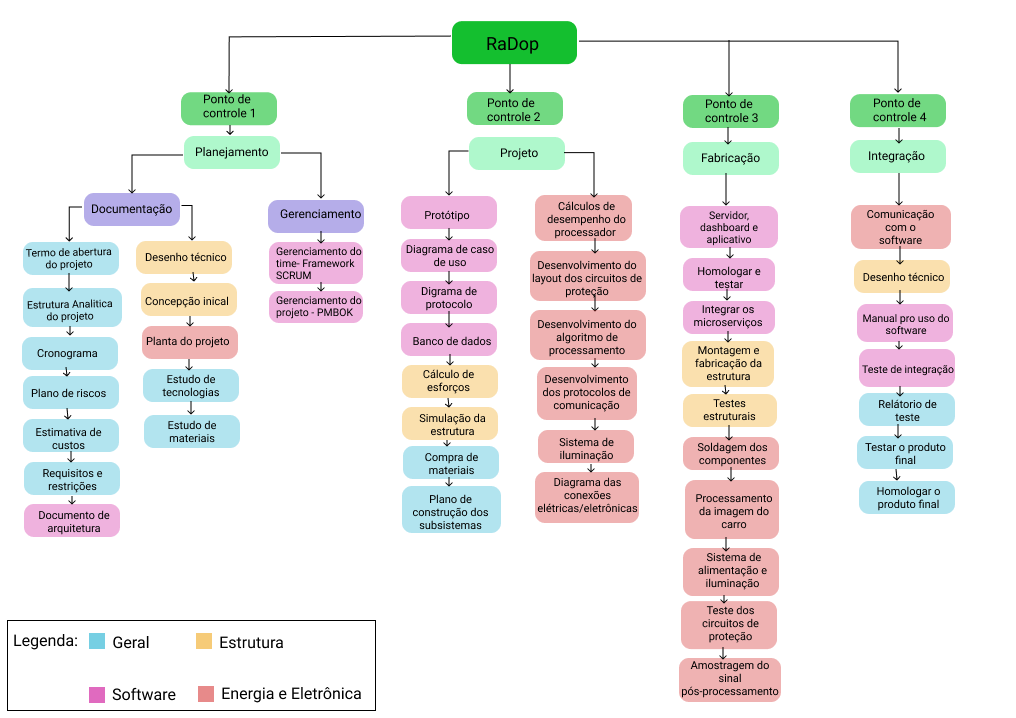
\includegraphics[width=\textwidth]{eap}}
    \caption{\label{fig:eap} EAP do projeto}
\end{figure}
\section{Lista É/Não é}
\subsection{É}
\subsection{Não é}
\section{Requisitos}
\subsection{Eletrônica}
\subsection{Energia}
\begin{itemize}
	\item O sistema deve conter painéis fotovoltaicos que promoverão a fonte de alimentação para todos os componentes do sistema;
	\item O sistema deve garantir o máximo aproveitamento energético;
	\item O sistema deve conter circuitos de controle de tensão e corrente;
	\item O sistema deve conter circuitos de controle de tensão e corrente;
	\item O sistema deve garantir o funcionamento seguro e contínuo do Radar;
	\item O sistema deve conter um circuito de iluminação para servir de alerta aos motoristas;
	\end{itemize
\subsubsection{Restrições}
\begin{itemize}
   \item Dependêcia do clima para a geração de energia;
   \item Localização Geografica;
   \item Temperatura média;
   \item Indices de radiação solar;
   \item Posicionamento das placas em relação a radiação solar;
   \item Horário de exposição;
   \item Existência de sombramento
 \end{itemize}
\subsection{Estrutura}
\subsection{Software}

Os requisistos de software são:

\begin{itemize}
    \item Interface do Dashboard;
    \item Interface do Aplicativo;
    \item Manual de uso dos softwares (Microsserviços, Aplicativo e Dashboard);
    \item Funcionar com conexão a redes (Internet);
    \item Ser capaz de lidar e recuperar de falhas e erros (conexão, processamento e etc.);
    \item Softwares devem ser manuteníveis e evolutíveis;
    \item Softwares devem ser testáveis e testados;
    \item Software deve mostrar dados e informações do Radar;
    \item Software deve ser capaz de tomar decisões para alertar socorristas a respeito de prováveis acidentes automobilísticos;
    \item Software deve ser capaz de tomar decisões para alertar usuários de possíveis situações de risco;
    \item Software deve ser capaz de mostrar informações gerenciais com os dados do Radar;
\end{itemize}

As restrições de software são:

\begin{itemize}
    \item O software necessita estar sempre conectado à internet para comunicação e, consequentemente, para o correto funcionamento;
    \item O aplicativo de manutenção irá auxiliar apenas com o essencial;
    \item O aplicativo só funcionará em aparelhos Android;
    \item A linguagem de cada microsserviço (assim como framework/tecnologia) será definida dada necessidade (performance, armazemanento e etc) dos mesmos;
\end{itemize}

\section{\emph{Stakeholders}}
\section{Recurso humanos}
\section{Cronograma de atividades}
\section{Milestones Identificados}
\section{Estimativa de custos}

\subsection{Engenharia de Software}

Aqui está listado todos os gastos que serão necessários para a equipe de software, assim como todas as aquisições que serão feitas durante o projeto:

\begin{table}[]
    \resizebox{\textwidth}{!}{\begin{tabular}{@{}|c|c|c|c|c|c|c|@{}}
    \toprule
    \textbf{Nome do produto} & \textbf{Descrição}                      & \textbf{Marca} & \textbf{Preço unitário} & \textbf{Quantidade} & \textbf{Fornecedor} & \textbf{Orçamento} \\ \midrule
    Servidor                 & Máquina para execução dos serviços      & ---            & US\$ 10,00 por mês      & 5 meses             & Digital Ocean       & US\$ 50,00         \\ \midrule
    Raspberry Pi 3 B         & Placa de IoT para execução de softwares & Raspberry      & R\$ 279,90              & 1 unidade           & FilipeFlop          & R\$ 279,90         \\ \bottomrule
    \end{tabular}}
\end{table}

OBS: Essa planilha poderá ser atualizado dependendo de necessidades que surgirem durante a execução do projeto.

\section{Viabilidades financeira}
\section{Levantamento de riscos}
\subsubsection{Energia}
\begin{itemize}
   \item Alimentação insuficiente ao Radar;
   \item Curta vida útil dos equipamentos; 
   \item Queima dos componentes elétricos;
   \item Tamanho da bitola dos cabos insuficiente para a quantidade de tensão e corrente;
   \item Montagem mal feita;
   \item Altura da fonte de alimentação segura para realizar manutenção e instalação;
   \item Pista movimentada no dia da instalação;
   \item Negligenciamento da dissipação de calor;
   \item Estrutura mal dimensionada para o suporte e proteção do sistema de alimentação
 \end{itemize}